\documentclass[11pt,a4paper]{report}

%%%%%%%%%%%%%%%%%%%%%%%%%%%%%%%%%%%%%%%%%%%%%%%%%%%%%%%%%%%%%%%%%%%%
%%-----------------------PAGE SETTINGS----------------------------%%
%%%%%%%%%%%%%%%%%%%%%%%%%%%%%%%%%%%%%%%%%%%%%%%%%%%%%%%%%%%%%%%%%%%%
\usepackage[utf8]{inputenc}
\usepackage[a4paper,top=1in,bottom=1in,left=1.15in,right=1.15in]{geometry}

%%%%%%%%%%%%%%%%%%%%%%%%%%%%%%%%%%%%%%%%%%%%%%%%%%%%%%%%%%%%%%%%%%%%
%%--------------------------PREAMBLE------------------------------%%
%%%%%%%%%%%%%%%%%%%%%%%%%%%%%%%%%%%%%%%%%%%%%%%%%%%%%%%%%%%%%%%%%%%%
\usepackage{graphicx}
\usepackage{pdfpages}
\usepackage{anyfontsize}
\usepackage{setspace}
\usepackage{amsmath}
\usepackage{amssymb}
\usepackage{amsthm}
\usepackage{titlesec}
\usepackage{xcolor}
\usepackage[colorlinks=true,linkcolor=blue,citecolor=blue,urlcolor=blue]{hyperref}
\newtheorem{theorem}{Theorem}[chapter]
\titleformat{\chapter}[hang]
{\normalfont\LARGE\bfseries}
{\thechapter}
{1em}
{}

\titlespacing*{\chapter}{0pt}{-10pt}{18pt}

\titleformat{\section}[hang]
{\normalfont\large\bfseries}
{\thesection}
{1em}
{}

\titlespacing*{\section}{0pt}{14pt}{8pt}

%%%%%%%%%%%%%%%%%%%%%%%%%%%%%%%%%%%%%%%%%%%%%%%%%%%%%%%%%%%%%%%%%%%%
%%-----------------------CUSTOM COMMANDS--------------------------%%
%%%%%%%%%%%%%%%%%%%%%%%%%%%%%%%%%%%%%%%%%%%%%%%%%%%%%%%%%%%%%%%%%%%%
\newcommand{\textBF}[1]{%
    \pdfliteral direct {2 Tr 1 w}
     #1%
    \pdfliteral direct {0 Tr 0 w}%
}

\newcommand{\textDF}[1]{%
    \pdfliteral direct {2 Tr 0.2 w}
     #1%
    \pdfliteral direct {0 Tr 0 w}%
}

%%%%%%%%%%%%%%%%%%%%%%%%%%%%%%%%%%%%%%%%%%%%%%%%%%%%%%%%%%%%%%%%%%%%
%%-----------------------DOCUMENT BEGIN---------------------------%%
%%%%%%%%%%%%%%%%%%%%%%%%%%%%%%%%%%%%%%%%%%%%%%%%%%%%%%%%%%%%%%%%%%%%
\begin{document}

\newgeometry{margin=0.01cm}
\begin{titlepage}
\thispagestyle{empty}
\title{

\includegraphics[width=19cm]{Extras/Mathlogo.PNG} \\
\vspace{3cm}
\begingroup
\fontsize{28}{34}\selectfont
\setstretch{1.05}
\parbox{15.5cm}{\textBF{Randomized approaches to approximating solutions of large kernel systems for Kernel Ridge Regression using the Nystr\"om method}}
\endgroup}
\date{}
\author{}
\maketitle
\vspace{-1.5cm}
\hspace{4cm}\parbox[b][15cm][b]{8cm}{\textDF{\large\setstretch{1.5}
Bachelor's Project Mathematics\\
April 2026\\
Student: Y. Tao\\
First supervisor: Dr. M. Meier\\
Second supervisor: Dr. A. Smith}}
\end{titlepage}
\restoregeometry
\clearpage

\chapter*{Abstract}
Kernel ridge regression leads to a linear system involving the full kernel matrix $K$. This matrix has size $n \times n$, so forming and storing it becomes expensive when the number of data points is large. This project studies randomized Nystr\"om approximations, where only $l \ll n$ columns of $K$ are used to build a low-rank approximation. The aim is to compare how the choice of sampled columns and the number of sampled columns affect accuracy, runtime, memory use, conditioning, and solver behaviour.

\clearpage

\tableofcontents

\clearpage

\chapter{Introduction}
Kernel methods provide a way to capture nonlinear relationships by projecting data onto a higher-dimensional space and describing the data through pairwise similarities. Kernel functions are used to compute inner products in the higher-dimensional space without explicitly mapping the data. This allows flexible regression models to be constructed, but the resulting matrix computations become expensive as the number of observations increases \citep{alaoui2015fast}. This project therefore studies randomized Nystr\"om approximation, one of the most popular techniques that reduces this computational cost for kernel ridge regression while trying to preserve its prediction quality \citep{musco2017recursive}. 

Many regression problems start with data $(x_i,y_i)$ for $i=1,\ldots,n$, where $n$ is the number of observations, $x_i\in\mathbb{R}^d$ are the inputs and $y_i\in\mathbb{R}$ are the outputs. We would like to use these data to create a model for the relationship between the inputs and outputs. One formulation of this task is kernel ridge regression, which uses a kernel function $k$ to measure pairwise similarities between the inputs. These values form the $n\times n$ kernel matrix $K$, whose entries are $K_{ij}=k(x_i,x_j)$. The details of this formulation are introduced in Chapter 2.

For large datasets, the main computational difficulty is the need to explicitly form the full matrix $K$, which costs $O(n^2)$ time and memory. This is the part that becomes infeasible first and takes the most time and resources. Solving the resulting system directly can also cost about $O(n^3)$ operations, so this is fine for small tests, but not realistic when $n$ becomes large \citep{drineas2005nystrom,alaoui2015fast}.

Therefore in this project we investigate the Nystr\"om approximation of the kernel matrix. Instead of forming all of $K$, we select an index set $I\subset\{1,\ldots,n\}$ containing $l\ll n$ column indices. The selected columns form the matrix $C=K_{:,I}\in\mathbb{R}^{n\times l}$, while their intersections with the corresponding rows form the smaller matrix $W=K_{I,I}\in\mathbb{R}^{l\times l}$. These two matrices are then used to construct a low-rank approximation $\tilde K\approx K$, for example $\tilde K = CW^\dagger C^T$. This is a randomized approach for kernel matrices \citep{drineas2005nystrom,gittens2013revisiting}. The point is to reduce the computational cost while still keeping enough information from the original kernel matrix. The full construction is introduced in Chapter 3.

Nystr\"om needs a set of $l$ columns to build $\tilde K$. The simplest choice is uniform random sampling, i.e. pick columns uniformly at random. Smarter strategies try to pick columns that are more informative so that fewer columns are needed for similar accuracy. One idea is to sample according to ridge leverage scores, which give higher probability to points that matter more for the kernel ridge regression solution \citep{alaoui2015fast}. Another idea is to approximate these leverage type probabilities adaptively without ever constructing the whole $K$ \citep{calandriello2017distributed}.

This project is therefore about how to decide which columns to sample and how many columns $l$ are needed for a good Nystr\"om approximation in the KRR setting. We will compare different sampling strategies, starting from uniform random sampling as a baseline, and then compare against smarter strategies motivated by the literature. The experiments will compare these strategies in terms of prediction accuracy and computational complexity, such as runtime and memory, as $l$ changes.

The research questions are:
\begin{itemize}
\item What Nystr\"om column sampling strategies give good performance for KRR in terms of prediction accuracy vs runtime/memory?
\item How large does $l$ need to be to get a good approximation, and how does this depend on the sampling strategy and $\lambda$?
\item What do the accuracy and cost (runtime/memory) trade-offs look like when $l$ increases, and can we recommend a reasonable approach?
\item How do conditioning and solver convergence relate to $\lambda$ and the Nystr\"om approximation quality?
\end{itemize}

This thesis is organised as follows. Chapter 2 introduces kernel ridge regression and the kernel matrices used in the project. It also gives the first singular value experiments, which motivate why a low-rank approximation is a reasonable thing to try. Chapter 3 introduces the Nystr\"om approximation, starting from the general positive semidefinite matrix formula and then moving to column sampling. 
\chapter{Kernel Ridge Regression}

\section{Introduction to the regression problem}

In this section we introduce the regression problem that will be used throughout the project. Assume we have a dataset $(x_i,y_i)$ for $i=1,\ldots,n$ where $x_i\in\mathbb{R}^d$ are inputs and $y_i\in\mathbb{R}$ are outputs. We would like to use these data to create a model for the relationship between the $x$ and $y$. In ordinary linear regression one searches over linear functions of the input variables. Kernel ridge regression instead searches over a reproducing kernel Hilbert space $\mathcal{H}$, which allows nonlinear functions to be represented through a kernel function.

Let
\[
k:\mathbb{R}^d\times\mathbb{R}^d\to\mathbb{R}
\]
be a positive definite kernel function. For the training data we define the kernel matrix
\[
K\in\mathbb{R}^{n\times n},\quad K_{ij}=k(x_i,x_j).
\]
The entry $K_{ij}$ measures the similarity between the data points $x_i$ and $x_j$ according to the chosen kernel function. The matrix $K$ induced by $k$ is symmetric positive semidefinite.

The kernel trick allows us to formulate this as
\[
\min_{f\in\mathcal{H}}\|f(X)-y\|_2^2+\lambda\|f\|_{\mathcal{H}}^2,
\]
which is also
\[
\min_{f\in\mathcal{H}}\sum_{i=1}^n(f(x_i)-y_i)^2+\lambda\|f\|_{\mathcal{H}}^2.
\]
Here $\lambda>0$ is the regularization parameter. The first term measures the error on the training data while the second term penalizes functions with large RKHS norm. Here $\lambda$ controls the trade off between fitting the data and overfitting.

\section{Representer form}

By the representer theorem, the minimizer has the form
\[
f(x)=\sum_{j=1}^n\alpha_j k(x,x_j),
\]
for some coefficient vector
\[
\alpha=(\alpha_1,\ldots,\alpha_n)^T\in\mathbb{R}^n.
\]
For the training points we have
\[
f(x_i)=\sum_{j=1}^n\alpha_j k(x_i,x_j),
\]
so in vector form
\[
f(X)=K\alpha.
\]
Therefore the data fitting term becomes
\[
\sum_{i=1}^n(f(x_i)-y_i)^2=\|K\alpha-y\|_2^2.
\]

The RKHS norm term can also be written using the kernel matrix. First, by the reproducing property,
\[
\langle k(\cdot,x_i),k(\cdot,x_j)\rangle_{\mathcal{H}}=k(x_i,x_j).
\]
Since
\[
f=\sum_{i=1}^n\alpha_i k(\cdot,x_i),
\]
we have
\[
\|f\|_{\mathcal{H}}^2=\left\langle\sum_{i=1}^n\alpha_i k(\cdot,x_i),\sum_{j=1}^n\alpha_j k(\cdot,x_j)\right\rangle_{\mathcal{H}}.
\]
Using bilinearity of the inner product,
\[
\|f\|_{\mathcal{H}}^2=\sum_{i=1}^n\sum_{j=1}^n\alpha_i\alpha_j\langle k(\cdot,x_i),k(\cdot,x_j)\rangle_{\mathcal{H}}.
\]
Using the reproducing property again,
\[
\|f\|_{\mathcal{H}}^2=\sum_{i=1}^n\sum_{j=1}^n\alpha_i\alpha_j k(x_i,x_j).
\]
Since $K_{ij}=k(x_i,x_j)$ this becomes
\[
\|f\|_{\mathcal{H}}^2=\alpha^T K\alpha.
\]
Substituting this into the objective gives
\[
\min_{\alpha\in\mathbb{R}^n}\|K\alpha-y\|_2^2+\lambda\alpha^T K\alpha.
\]
Expand
\[
\|K\alpha-y\|_2^2=(K\alpha-y)^T(K\alpha-y).
\]
Then differentiate
\[
(K\alpha-y)^T(K\alpha-y)+\lambda\alpha^T K\alpha
\]
with respect to $\alpha$. Since $K$ is symmetric this gives
\[
2K(K\alpha-y)+2\lambda K\alpha=0.
\]
This then reduces to
\[
(K+\lambda I)\alpha=y.
\]
Therefore the coefficient vector is
\[
\alpha=(K+\lambda I)^{-1}y.
\]
The prediction for a new point $x$ is then
\[
\hat f(x)=\sum_{j=1}^n\alpha_j k(x,x_j).
\]
If $X_{\text{test}}$ is a set of test points and $K_{\text{test},\text{train}}$ is the matrix with entries
\[
(K_{\text{test},\text{train}})_{ij}=k(x_i^{\text{test}},x_j^{\text{train}}),
\]
then the test predictions are
\[
\hat y_{\text{test}}=K_{\text{test},\text{train}}\alpha.
\]

The regularization term is important numerically. Since $K$ can have very small eigenvalues or even zero eigenvalues, adding $\lambda I$ shifts all eigenvalues by $\lambda$ so $K+\lambda I$ is positive definite. This makes the system uniquely solvable and improves the conditioning of the problem.

For large datasets, the main computational difficulty is that $K$ is an $n\times n$ matrix. Forming the full kernel matrix requires $O(n^2)$ kernel evaluations and storing it requires $O(n^2)$ memory. Solving the system directly, for example by Cholesky decomposition, costs $O(n^3)$ operations. For small $n$ this is fine but for large datasets this quickly becomes infeasible. Therefore in this project we investigate the Nystr\"om approximation of the kernel matrix: instead of forming all of $K$, we only form $l\ll n$ sampled columns and the corresponding $l\times l$ submatrix, and then make a low rank approximation $\tilde K\approx K$.

\section{Kernel choices}

In the experiments we start with three common kernels. The linear kernel is
\[
k(x,z)=x^Tz.
\]
The polynomial kernel used in the first tests is
\[
k(x,z)=(x^Tz+1)^2.
\]
The Gaussian radial basis function kernel (rbf) is
\[
k(x,z)=\exp(-\gamma\|x-z\|_2^2).
\]
The parameter $\gamma$ controls how local the Gaussian kernel is. Larger $\gamma$ makes points only strongly similar to very nearby points while smaller $\gamma$ makes the similarities decay more slowly.

\section{Singular values and low-rank structure}

A kernel matrix is useful for Nystr\"om approximation when its singular values decay. If many singular values are very small then much of the matrix can be approximated using a smaller rank. This is why in this section we look at singular values of $K$ for real data. The point is to check whether a low-rank approximation is reasonable for real world data.

For this real data experiment we use the Superconductivity dataset from the UCI Machine Learning Repository. This is a regression dataset with $21263$ samples and $81$ numerical input features, and the output is the critical temperature. This fits the KRR setting since the target variable is continuous.

This dataset is also large enough to show the computational problem. If the full dataset is used, the kernel matrix has size
\[
21263\times 21263.
\]
This means there are
\[
21263^2=452115169
\]
entries in $K$. If these entries are stored in double precision, then just storing one dense kernel matrix takes about
\[
452115169\cdot 8\text{ bytes}\approx 3.6\text{ GB}.
\]
This is before solving the linear system or computing any decomposition. So the full matrix is already expensive, and this is the reason that an approximation method such as Nystr\"om is relevant.

The first singular value experiment uses the linear kernel
\[
k(x,z)=x^Tz.
\]
For a data matrix $X\in\mathbb{R}^{n\times d}$, this gives
\[
K=XX^T.
\]
In the Superconductivity dataset $d=81$, so the linear kernel matrix satisfies
\[
\operatorname{rank}(K)\leq 81.
\]
Therefore for the linear kernel, at most $81$ singular values can be nonzero. This is a simple case where the low-rank structure is built into the kernel matrix. It is still a useful first check because it shows directly how the dimension of the data can limit the rank of $K$.

\begin{figure}[h]
\centering
\IfFileExists{Results/sing_vals_linear_kernel.pdf}{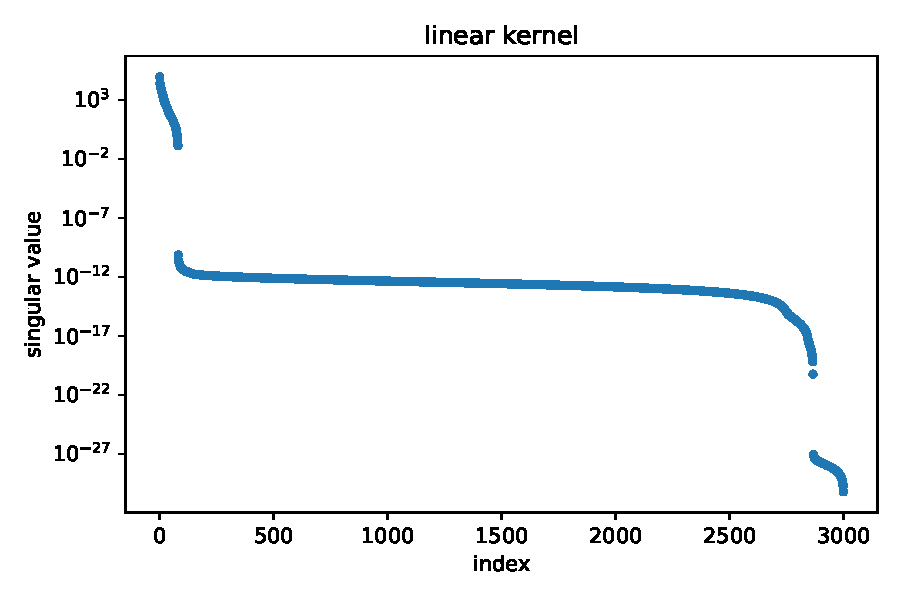
\includegraphics[width=0.75\textwidth]{Results/sing_vals_linear_kernel.pdf}}{\fbox{Run the singular value experiment to create this figure}}
\caption{Singular values of a kernel matrix from the Superconductivity dataset using the linear kernel.}
\label{fig:singular-linear}
\end{figure}

I also compare this with the Gaussian RBF kernel
\[
k(x,z)=\exp(-\gamma\|x-z\|_2^2).
\]
For this kernel the rank is not limited by $d$ in the same simple way. The singular value decay depends on the geometry of the data and on the parameter $\gamma$. This makes the RBF kernel more interesting for checking whether the singular values still decay in practice.

\begin{figure}[h]
\centering
\IfFileExists{Results/sing_vals_rbf_kernel.pdf}{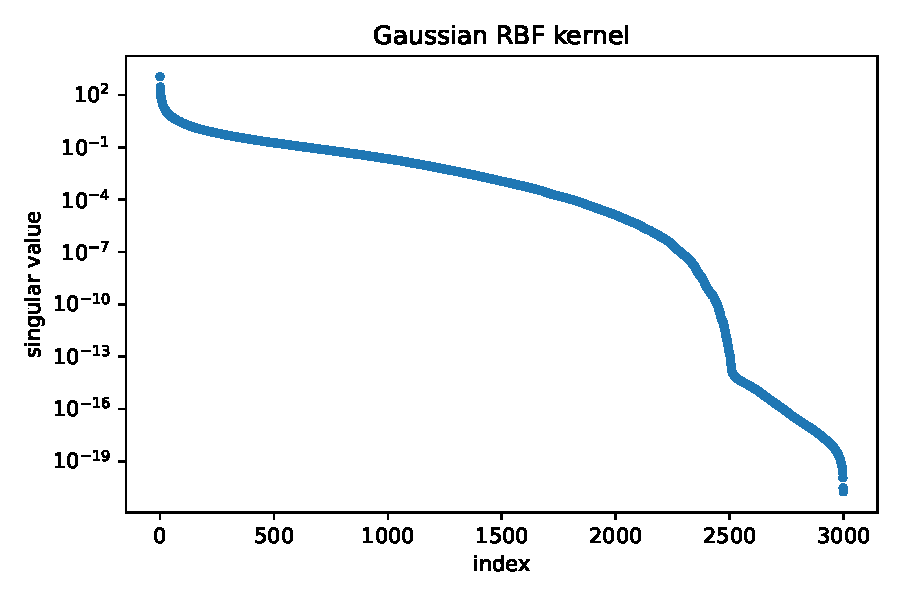
\includegraphics[width=0.75\textwidth]{Results/sing_vals_rbf_kernel.pdf}}{\fbox{Run the singular value experiment to create this figure}}
\caption{Singular values of a kernel matrix from the Superconductivity dataset using the Gaussian RBF kernel.}
\label{fig:singular-rbf}
\end{figure}
\chapter{Nystr\"om Approximation}

The Nystr\"om method is a way to approximate a large positive semidefinite matrix by using only a smaller part of it. In this project the positive semidefinite matrix is the kernel matrix $K$, but it is useful to first describe the construction for a general positive semidefinite matrix $A$. The aim is to build a low rank approximation $\tilde{A}$ without using all of $A$ in a full direct factorization.

\section{General Nystr\"om form}

Following the general formulation in randomized numerical linear algebra, let
\[
A\in\mathbb{R}^{n\times n},\quad A\succeq0,
\]
and let
\[
X\in\mathbb{R}^{n\times l}
\]
be a test matrix, the Nystr\"om approximation of $A$ with respect to $X$ is
\[
A\langle X\rangle=(AX)(X^TAX)^\dagger(AX)^T.
\]
Here $(X^TAX)^\dagger$ denotes the Moore--Penrose pseudoinverse. The matrix $AX$ contains the information we collect from $A$. The smaller matrix
\[
X^TAX\in\mathbb{R}^{l\times l}
\]
describes how the sampled directions interact with each other. This is the same general positive semidefinite sketching model used by Gittens and Mahoney, where one forms $C=AS$, $W=S^TAS$, and then uses $CW^\dagger C^T$ as the approximation \cite{gittens2016nystrom}.

This formula shows why the approximation has rank at most $l$ since the formula is a product involving the $n\times l$ matrix $AX$, so
\[
\operatorname{rank}(A\langle X\rangle)\leq l.
\]
Therefore, when $l\ll n$, the approximation is much cheaper to store and compute with than the full matrix $A$.

There is also a useful geometric representation of this formula. Since $A$ is positive semidefinite we can use $A^{1/2}$. Then
\[
A\langle X\rangle=A^{1/2}P_{A^{1/2}X}A^{1/2},
\]
where $P_{A^{1/2}X}$ is the orthogonal projector onto the column space of $A^{1/2}X$. This has error as
\[
A-A\langle X\rangle=A^{1/2}(I-P_{A^{1/2}X})A^{1/2}
\]
which is the Schur complement viewpoint used by Martinsson and Tropp \cite{martinsson2021randomized}. This means that the Nystr\"om approximation keeps the part of $A$ which is seen through the subspace generated by $X$.

\begin{theorem}
Let $A\in\mathbb{R}^{n\times n}$ be positive semidefinite and let $X\in\mathbb{R}^{n\times l}$. Then
\[
A-A\langle X\rangle=A^{1/2}(I-P_{A^{1/2}X})A^{1/2}.
\]
In particular,
\[
A-A\langle X\rangle\succeq0,
\]
so
\[
0\preceq A\langle X\rangle\preceq A.
\]
\end{theorem}

\begin{proof}
Let
\[
Z=A^{1/2}X.
\]
The orthogonal projector onto the column space of $Z$ is
\[
P_Z=Z(Z^TZ)^\dagger Z^T.
\]
Since $Z=A^{1/2}X$, we have
\[
Z^TZ=X^TAX.
\]
Therefore
\[
A^{1/2}P_ZA^{1/2}=A^{1/2}A^{1/2}X(X^TAX)^\dagger X^TA^{1/2}A^{1/2}.
\]
This gives
\[
A^{1/2}P_ZA^{1/2}=(AX)(X^TAX)^\dagger(AX)^T=A\langle X\rangle.
\]
Hence
\[
A-A\langle X\rangle=A^{1/2}IA^{1/2}-A^{1/2}P_ZA^{1/2}=A^{1/2}(I-P_Z)A^{1/2}.
\]
Since $I-P_Z$ is an orthogonal projector, it is positive semidefinite. Thus
\[
A-A\langle X\rangle\succeq0.
\]
This also gives
\[
0\preceq A\langle X\rangle\preceq A.
\]
\end{proof}

This is useful because it says that the Nystr\"om approximation does not create a matrix larger than $A$ in the positive semidefinite order. It approximates $A$ from below. In the KRR setting this matters because replacing $K$ by $\tilde K$ changes the regularized system from
\[
(K+\lambda I)\alpha=y
\]
to
\[
(\tilde K+\lambda I)\tilde\alpha=y.
\]
Since $\tilde K\preceq K$, the approximation changes both the estimator and the conditioning of the linear system. This is one reason why the number of sampled columns $l$, the sampling strategy and the regularization parameter $\lambda$ have to be studied together.

\section{Column sampling}

We now look at column sampling. Let
\[
I=\{i_1,\ldots,i_l\}\subset\{1,\ldots,n\}
\]
be the selected column indices. Define the sampling matrix
\[
S=\begin{bmatrix}e_{i_1}&e_{i_2}&\cdots&e_{i_l}\end{bmatrix}\in\mathbb{R}^{n\times l},
\]
where $e_i$ is the $i$-th standard basis vector. Taking $X=S$ in the general Nystr\"om formula gives
\[
\tilde K=K\langle S\rangle=(KS)(S^TKS)^\dagger(KS)^T.
\]
Now define
\[
C=KS=K_{:,I}\in\mathbb{R}^{n\times l}
\]
and
\[
W=S^TKS=K_{I,I}\in\mathbb{R}^{l\times l}.
\]
Then the Nystr\"om approximation becomes
\[
\tilde K=CW^\dagger C^T.
\]
Equivalently,
\[
\tilde K=K_{:,I}(K_{I,I})^\dagger K_{I,:}.
\]
This is the form used in this project. Instead of forming or storing all of $K$, the approximation is built from the sampled columns $K_{:,I}$ and the smaller intersection matrix $K_{I,I}$. If $W$ is invertible then the formula simplifies to
\[
\tilde K=CW^{-1}C^T.
\]
However in practice $W^\dagger$ is safer to write since $W$ can be singular or nearly singular.

The computational meaning is obviously seen. The full kernel matrix has $n^2$ entries. The column sampling form only needs the $n\times l$ matrix $C$ and the $l\times l$ matrix $W$. So the storage goes from order $n^2$ to order $nl+l^2$. This becomes significantly useful when $l\ll n$.

\section{Randomized Nystr\"om approximation}

The randomized Nystr\"om approximation draws a random matrix
\[
\Omega\in\mathbb{R}^{n\times l}
\]
and form
\[
Y=A\Omega.
\]
Then the Nystr\"om approximation is
\[
\hat A=Y(\Omega^TY)^\dagger Y^T.
\]
This is the randomized Nystr\"om approximation described by Martinsson and Tropp \cite{martinsson2021randomized}. The idea is that the random matrix $\Omega$ collects information about the important directions of $A$. If the column space of $A\Omega$ captures the dominant eigenspace of $A$ well then the approximation error should be small.

For kernel matrices the usual Nystr\"om method samples columns of $K$. This corresponds to taking $\Omega=S$, where $S$ is a column selection matrix. Then
\[
Y=KS=K_{:,I},
\]
and the formula becomes
\[
\tilde K=K_{:,I}(K_{I,I})^\dagger K_{I,:}.
\]
Thus in this project randomness enters through the random choice of the index set $I$. Different choices of the distribution for $I$ give different Nystr\"om methods.

\section{Uniform sampling}

The baseline method is uniform sampling. This means choosing $l$ column indices from $\{1,\ldots,n\}$ uniformly at random. It is easy to implement and cheap because no importance scores have to be computed. Its weakness is that it treats all columns equally. If some columns are much more informative than others, uniform sampling may need a larger $l$ to reach the same accuracy as a smarter strategy.

Before stating the theorem for this, we need the idea of coherence. Let $K$ be a positive semidefinite kernel matrix and let $K=U\Lambda U^T$ be its eigendecomposition. Let $U_k\in\mathbb{R}^{n\times k}$ contain the leading $k$ eigenvectors. The leverage score of row or column $i$ relative to this $k$-dimensional eigenspace is $s_i=\|U_k(i,:)\|_2^2.$
These scores satisfy $\sum_{i=1}^n s_i=k.$

This measures how concentrated the leading eigenspace is in a few rows. If the scores are all similar, then $\mu$ is not large and uniform sampling has a better chance of working. If a few scores are much larger than the rest, then uniform sampling can easily miss important columns.

This issue is discussed by Gittens and Mahoney. In some datasets the leverage scores are fairly uniform so uniform sampling can be reasonable. In other datasets the leverage scores are highly nonuniform and uniform sampling can be much worse \cite{gittens2016nystrom}. This is why uniform sampling is a natural baseline method but not necessarily the best method.

\begin{theorem}[Uniform sampling and coherence]
Let $K\in\mathbb{R}^{n\times n}$ be positive semidefinite, and let $K_k$ be its best rank $k$ approximation. Fix a failure probability $\delta$ and an accuracy factor $\epsilon$ both in $(0,1)$. Suppose $l$ columns are sampled uniformly at random. In the basic Nystr\"om method we are using here, this corresponds to the $q=1$ case of Lemma 8 in Gittens and Mahoney, so
\[
C=KS=K_{:,I},\qquad W=S^TKS=K_{I,I}.
\]
If
\[
l\geq 2\mu\epsilon^{-2}k\ln(k/\delta),
\]
then, with probability at least $1-3\delta$, the Nystr\"om approximation $\tilde K=CW^\dagger C^T$ satisfies the spectral norm bound
\[
\|K-\tilde K\|_2 \leq \left(1+\frac{n}{(1-\epsilon)l}\right)\|K-K_k\|_2.
\]
\end{theorem}

This bound for $l$ fits the intuition as it shows us when $\mu$ is large we need to sample more columns. This is exactly the point that uniform sampling does not know which columns are important so when the coherence is large it needs more columns to capture the essential structure.

In the first experiments we test uniform sampling. For each $l$, the approximation quality can be measured directly by a relative forward error, for example
\[
\frac{\|K-\tilde K\|_F}{\|K\|_F}.
\]
It is also important to measure the effect on prediction. So the approximation is also judged by what happens when $\tilde K$ is used in place of $K$ in the regularized system, this is done by solving the system with $\tilde K$ and then measuring the test error of the result.

\section{Leverage score sampling}

Uniform sampling is cheap but it ignores the structure of $K$. Leverage score sampling is the opposite extreme, it tries to sample columns according to how important they are in the leading eigenspace.

The full leverage score version is the most informed method. It uses all of $K$ first:
\begin{enumerate}
\item construct the full kernel matrix $K$;
\item compute the leading eigenvectors $U_k$;
\item compute the squared row norms $s_i=\|U_k(i,:)\|_2^2$;
\item compute probabilities $p_i=\frac{s_i}{\sum_j s_j}$;
\item sample columns according to these probabilities.
\end{enumerate}

This method is expensive because it requires the full matrix and the leading eigenvectors. But it is still useful as a reference method. It says what the informed sampling distribution would be if the important eigenspace was already known.

\begin{theorem}[Leverage score sampling]
Let $K\in\mathbb{R}^{n\times n}$ be positive semidefinite and let $U_k$ contain the leading $k$ eigenvectors. Suppose columns are sampled with probabilities satisfying
\[
p_i\geq\frac{\beta}{k}\|U_k(i,:)\|_2^2
\]
for some $\beta\in(0,1]$. If the number of sampled columns has order
\[
l=O\left(\frac{k\log(k/\beta)}{\beta\epsilon^2}\right),
\]
then the Nystr\"om approximation satisfies 
\[
\|K-\tilde K\|_2 \leq \|K-K_k\|_2+\epsilon^2\|K-K_k\|_*,
\]
where $\epsilon$ is a fixed approximation factor.
\end{theorem}

The important thing here is the dependence on $l$. Uniform sampling has a coherence factor while leverage score sampling samples according to the row norm scores. This can cause leverage score sampling to use much fewer columns when the leverage scores are very uneven.

\section{Approximate leverage score sampling}

The full leverage score method is too expensive if the whole reason for Nystr\"om is to avoid working with all of $K$. The middle method is therefore to look at a small part of $K$ first and use it to estimate which rows or columns look important.

Here is a simple version of this idea:
\begin{enumerate}
\item sample $5$ columns uniformly;
\item form the small sampled matrix $K_s\in\mathbb{R}^{n\times 5}$;
\item compute an orthonormal basis $U_s$ for the column space of $K_s$;
\item compute approximate scores as before.
\item sample $95$ more columns (total $100$ columns) according to these approximate scores.
\end{enumerate}



\clearpage

\begin{thebibliography}{99}

\bibitem[Calandriello et al.(2017)]{calandriello2017distributed} Calandriello, D., Lazaric, A., and Valko, M. (2017). Distributed adaptive sampling for kernel matrix approximation. In \emph{Proceedings of the 20th International Conference on Artificial Intelligence and Statistics}.

\bibitem[Drineas and Mahoney(2005)]{drineas2005nystrom} Drineas, P. and Mahoney, M. W. (2005). On the Nystrom method for approximating a Gram matrix for improved kernel-based learning. \emph{Journal of Machine Learning Research}, 6, 2153--2175.

\bibitem[El Alaoui and Mahoney(2015)]{elalaoui2015fast} El Alaoui, A. and Mahoney, M. W. (2015). Fast randomized kernel methods with statistical guarantees. In \emph{Advances in Neural Information Processing Systems}.

\bibitem[Gittens and Mahoney(2016)]{gittens2016nystrom} Gittens, A. and Mahoney, M. W. (2016). Revisiting the Nystrom method for improved large-scale machine learning. \emph{Journal of Machine Learning Research}, 17, 1--65.

\bibitem[Martinsson and Tropp(2020)]{martinsson2021randomized} Martinsson, P.-G. and Tropp, J. A. (2020). Randomized numerical linear algebra: foundations and algorithms. \emph{Acta Numerica}.

\bibitem[Zhu(2025)]{zhu2025rkhs} Zhu, R. (2025). Reproducing kernel Hilbert space. \emph{Statistical Machine Learning with R}.

\bibitem[Hamidieh(2018)]{hamidieh2018superconductivity} Hamidieh, K. (2018). Superconductivty Data. UCI Machine Learning Repository. DOI: 10.24432/C53P47.

\end{thebibliography}

\end{document}